% !TeX root = ../DistributedConsensus.tex
% !TeX spellcheck = en_GB
\chapter{Background}\label{chap:background}
	\section{Dynamic Condition Response Graphs}\label{sec:background:dcrgraphs}
	Dynamic Condition Response Graphs (DCR graphs) is a declarative, event-based process model. Instead of using sequences of state transitions like imperative process languages, declarative process languages uses sets of constraints to model the possible transitions in the process (hereafter \textit{workflow}). A benefit of DCR graphs is that they allow finite specifications of infinite behaviour.

%	Since events in a DCR graphs are distributed and no algorithm for finding the order of execution currently exists, DCR graphs are well suited for developing an algorithm for determining history. 
%	Furthermore DCR graphs specify several types of directed edges in the graph, which provide useful information for determining order of execution.
	
	\newpar A DCR graph is in \cite{hildebrandt2011declarative} defined as a tuple $(E, M, Act, $\condition$, $\response$, \pm, l)$ where
	\begin{itemize}
		\item $E$ is the set of events
		\item $M$ is the marking, the state of the workflow. The marking is a triple containing three sets of events. The first set contains the events that have previously been executed. The second set contains the events that are required to be executed or excluded. These are called the pending responses. The last set contains the events which are currently included.
		\item $Act$ is the set of actions. That is, a representation of what happens in the workflow when a given event is executed.
		\item \condition (conditions) is a relation, which for all pairs of events which is present in the relation, means that the first event must be either excluded or executed for the second event to be executable.
		\item \response (responses) is a relation, which for all pairs of events which is present in the relation, means that after the first event has been executed the second event must either be executed or excluded at some point.
		\item $\pm$ defines the dynamic inclusion and exclusion of events. This partial function is a triple of two events and symbol defining whether the execution of the first event should result in an exclusion or inclusion of the second event. It is possible for an event to exclude itself, but one event cannot both include and exclude another.
		\item $l$ is the labelling function, assigning an action to each event.
	\end{itemize}
		
	Furthermore the article defines a distributed DCR graph as a DCR graph with a set of roles, a set of principals, and a mapping function that assigns roles to principals and actions. This assignment means that if principal $P$ is assigned role $R$, and action $A$ is assigned $R$, then $P$ can execute $A$.
		
	\newpar
	Events can be safely distributed by defining \textit{projections} and \textit{compositions} of DCR graphs. This is described in \cite{hildebrandt2011safe}.
	
	\newpar
	A projection of a DCR graph with respect to a subset of events of the graph and a subset of the labels of the graph. The label set must contain the labels of the events in the event set, as well as all labels of events that can affect the marking or the ability to execute an event in the projection, through relations.\figuretodo{If this should be kept, there should be a figure representing the projection of a graph.}
	
	\newpar
	Proposition 1 in \cite{hildebrandt2011safe} defines how an execution in a projection corresponds to the execution of events in the entire DCR graph the projection was made on. In short it describes if and how a transition in the projection corresponds to a transition in the entire DCR graph and vice versa.
	
	\newpar
	The composition of two DCR graphs defines the rules for how these graphs can be glued back together. The requirement is to keep all events and relations as well as combining the markings in a consistent manner. These rules can be found in definition 5 of \cite{hildebrandt2011safe}.
	\todo[inline]{Til Søren: da du henviste os til \cite{hildebrandt2011safe}, var det så Projection og Compositions du vil have os til at se på? Vi har lidt svært ved at se hvordan vi skal bruge denne del i resten af rapporten. (Vi har også lidt svært ved at forstå det) - Sørens svar: "[9:21] Ja, Projections og Compositions. I behøver ikke gøre et stort nummer ud af det, men i bør nævne, at i benytter essentielt den samme ide som i den artikel."}
    
	\newpar 
	In \cite{debois2015concurrency} Debois et al. describes the procedure for executing distributed events using a locking mechanism to ensure serial equivalence:
	
	\begin{quotation}
		The procedure for executing an event, in detail, is as follows. A component
		wishing to execute an event $e$ must first request\footnote{All components request locks in the same fixed order to prevent deadlocks.} and receive locks on all (local
		and remote) events that are in conflict (i.e., not independent ) with $e$ (thus, in
		particular, on itself). It then queries the state of remote events to determine if
		$e$ is currently executable. If it is, it instructs remote events affected by firing $e$
		to change state accordingly. Finally, it releases all locks.
	\end{quotation}
%	\newpar For example the events \textit{"Begin production"} and \textit{"Production finished"} can represent the start and end of the activity \textit{"Produce item X"}, which is an activity possibly containing several events. An event \textit{"Accept draft"}, can also represent a decision made or the event \textit{"Change password"} can represent an atomic event.
	
%	A DCR graph can model a \textit{workflow}, which represents a work process. The DCR graph can then be used to represent the current state of the process, to see what parts of the process have been completed and what parts of the process remain to be completed or \textit{executed}. 
	
%	The partitioning of the five types of relations in DCR graph makes modelling interconnected events possible, e.g. having an event in a process that makes another event non-executable. This is made possible by the \textit{exclusion} (\exclusion) relation, that excludes the other event and therefore makes in non-executable. 
	
%	Modeling an event that is dependent on the completion of another event is made possible by the \textit{condition} (\condition) relation, which makes it impossible to execute an event, unless the event that has a condition to it has been executed.
	
%	Modeling an event that can be excluded and then then re-included is made possible by the \textit{inclusion} (\inclusion) relation. 
	
%	Modeling an event that has to be executed in order for the event to be in an accepting state \todo{Find bedre phrasing for 'accepting'.} is made possible by the \textit{response} (\response) relation. If an event has a \textit{response} edge going to it in the DCR graph, the event is in a \textit{pending} state. The pending state signifies that the event should be executed in order for the process to be in an accepting state.
	
%	Users of a given DCR graph will execute events in order to change the state of the process the DCR graph is modelling. Events will have been executed in a certain order, which have resulted in the current state of the workflow. Several users can execute events concurrently in different locations. The events change state accordingly by communicating with reachable events. 
	
%	The implementation of a distributed system functioning as a DCR graph used in this project does not support the milestone relation.
			
	\section{Directed Graphs}
	A \textit{directed graph} is a data structure, which consists of \textit{nodes} connected by \textit{edges}. In directed graphs an edge is an ordered pair of nodes, where the first element is the start node and the second is the end node. When traversing the graph it is only possible to traverse edges from their start node to their end node. There exists a \textit{path} from a node to another if it is possible through one or more edges to get from the first to the second node.
	
	For a given node the \textit{reachability} is the set of all the nodes there exists a path to. For a graph to be \textit{acyclic} the reachability of all the nodes of the graph must not include the nodes themselves. 
	
	The subgraph of a given graph with the same reachability of each node, but with as few edges as possible, is called the \textit{minimum equivalent graph}.
	
	A \textit{topological order} of a directed graph is a linear ordering of the nodes, such that for every edge $a,b$ from node $a$ to $b$, $a$ comes before $b$.
	

	\section{Distributed Systems}
		Distributed systems is an area of computer science which focuses on the concepts, problems and design of computer systems where message transmission among processes are not negligible compared to the time between events in a single process. Traditionally these systems are distributed on computers in a network \cite{Lamport:1978:TCO:359545.359563}.
		
		\subsection{Serial Equivalence}
		Operations performed by two concurrent processes are serially equivalent if the resulting system state is the same as if any one of the processes' operation happened first, followed by the other. In distributed systems this term is used for transactions across machines in a network and is especially important since message passing over network connections introduce inconsistent and unpredictable delays. Therefore multiple messages can arrive at different times, even if they were supposed to happen in extension of one another. Common implementations of achieving serial equivalence in distributed systems include locking and optimistic concurrency control. In \cite{Coulouris:2011:DSC:2029110:chapter16} these concepts are explored in depth.
		
		\begin{figure}[H]
		\centering
		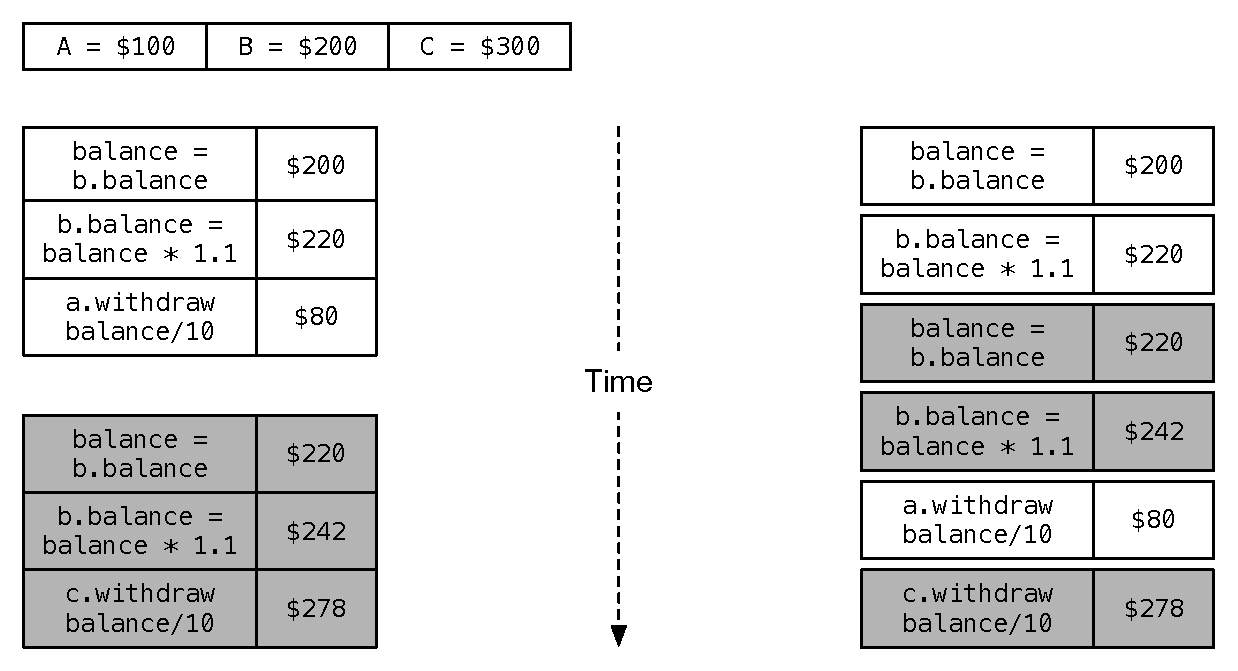
\includegraphics[width=\textwidth]{2background/images/serial-equivalence.pdf}
		\caption{Two transactions executed in sequence and a serially equivalent interleaving.}
		\label{fig:background:serial-equivalence}
		\end{figure}
		
		\subsection{Ordering of Events}\label{subsec:orderingofevents}
		In \cite{Lamport:1978:TCO:359545.359563} Leslie Lamport examines and describes the ordering of events (not to be confused with DCR events) in distributed systems based on their occurrence in time. Applying these concepts is very helpful when determining the order of execution in a DCR graph. 
		
		\newpar In set theory a total order is an order that is \textit{antisymmetric}, that is if $a \leq b$ and $b \leq a$ then $a = b$, as well as \textit{transitive}, that is if $a \leq b$ and $b \leq c$ then $a \leq c$, in addition to being \textit{total}, that is $a \leq b$ or $b \leq a$. For a total order to be strict the \textit{irreflexivity} property must also be present, that is $a \not< a$. A \textit{strict partial order} is similar to a \textit{strict total order} in that a strict partial order also has the \textit{transitive}, \textit{antisymmetry} and \textit{irreflexivity} properties, but not the \textit{totality} property.\figuretodo{Man kunne godt stille nogle små figurer op ved siden af hinanden der visualiserede de her properties.}
		
		These orders can be described with two examples, using a subset of the natural numbers, $\{1, 2, 3, 4, 5, 6\}$ referred to as $N$. 
		
		An example of a strict total order is $N$ ordered by the less-than ($<$) relation. An example of a strict partial order is $N$ ordered by the divisibility of the numbers, where the result of the division would be a natural number. An illustration of these two orders can be found seen on \autoref{fig:background:strict-partial} and \autoref{fig:background:strict-total}.
	
		\begin{figure}[H]
		\centering
		\begin{minipage}{0.45\textwidth}
			\centering
			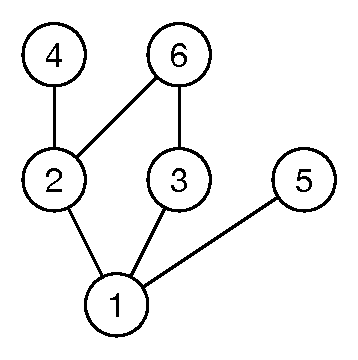
\includegraphics[height=\textheight/5]{2background/images/strict-partial.pdf}
		\caption{The strict partial order of $N$ ordered by divisibility resulting in a natural number. $A$ $\rightarrow$ $B$ denotes $A$ divides $B$.}
		\label{fig:background:strict-partial}
		\end{minipage}\hfill
		\begin{minipage}{0.45\textwidth}
			\centering
			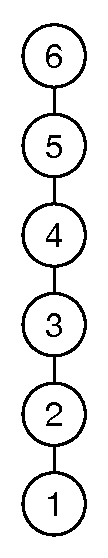
\includegraphics[height=\textheight/5]{2background/images/strict-total.pdf}
		\caption{The strict total order of the set of $N$ ordered by the less-than ($<$) relation.}
		\label{fig:background:strict-total}
		\end{minipage}
		\end{figure}
		
		\newpar Lamport introduces so-called \textit{logical clocks}, which are simple timestamps, that enable determining the order of events in a distributed system. The clocks are \textit{logical} in the sense that they do not represent \textit{physical} time, since synchronising time in a distributed system is a non-trivial task. A logical clock is a simple counter, that is incremented for each event happening in a process. 
		
		When a process receives a message, the counter must be set to a higher value than both the received timestamp, as well as the local clock. This also implies that each message must include the timestamp of the sending event. This is illustrated in \autoref{fig:background:lamport-timestamps}
		
		\begin{figure}[H]
		\centering
		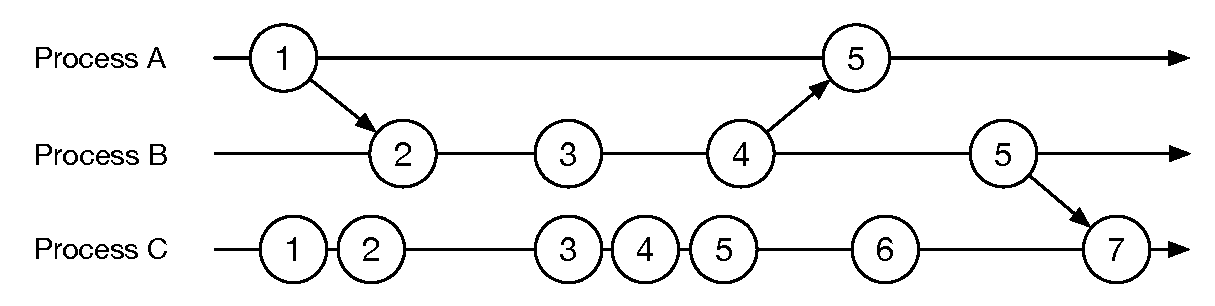
\includegraphics[width=\textwidth]{2background/images/lamport-timestamps.pdf}
		\caption{Three processes exchanging messages and setting their local timestamps accordingly.}
		\label{fig:background:lamport-timestamps}
		\end{figure}
		
		\newpar Lamport argues that if a given system is not distributed, it is possible to create a history of events where the ordering is total, since it is possible for one process to use a logical clock to find out which event happened before another. In a distributed system however, this global ordering is not possible, since events have independent locical clocks that can have the same timestamp.
		
		\newpar Lamport describes these relations between events with the symbol $\rightarrow$ such that if $event$ $a$ happened before $event$ $b$ then $a \rightarrow b$. These relations can be created based on three cases; The first case: if $event$ $a$ and $b$ happened on the same process and $a$ happened before $b$ measured with the local logical clock then $a \rightarrow b$. The second case: if process $i$ sends a message to process $j$ and $event$ $a$ is the event which initiates the sending and $event$ $b$ is the recieving of the message then $a \rightarrow b$. The third case is based on the transitive property such that if $a \rightarrow b$ and $b \rightarrow c$ then $a \rightarrow c$. If no relation exists between any event $a$ and $b$, the events are \textit{concurrent}, and logically occur at the same time, even though this might not be the case physically. Lamport therefore argues that it is only possible to find a partial order of events.\figuretodo{Disse happens before forhold kan også vises på en figur.}
		
		%\newpar Lamport then introduces a function $C_i(event)$ where $C_i$ is the clock function on process $i$ that if $a \rightarrow b$ then $C_i(a) < C_i(b)$. This clock can then be used to describe in values which event happened first. \todo{maybe this section is not neccesary. Or maybe it needs to be introduced before}
		
		\subsection{Consensus}
		Traditionally consensus in distributed systems is the activity of reaching agreement among the participants in the system on a proposed value. In \todo{disitrbuted systems bog side 669 kapitel 15} the consensus problem has the following three requirements:
		\begin{itemize}
			\item Termination: Eventually each correct process sets its decision variable
			\item Agreement: The decision value of all correct processes is the same
			\item Integrity: If the correct processes all proposed the same value, then any correct process in the decided state has chosen that value
		\end{itemize}
		
		\newpar Such problems are often achieved by using an consensus algorithm such as Paxos\cite{Lamport:1998:PP:279227.279229}, Raft \cite{Raft:Ongaro:184040} etc.
		
		Assumptions about the distributed system are made for Paxos and Raft, namely, processes operate at an arbitrary speed, may experience failures, may recover after a crash by storing their state, and do not collude, lie or attempt to subvert the protocol - in short: byzantine failures do not occur.
		
		In our problem domain processes may operate at an arbitrary speed, may experience failures, \textit{cannot} recover from a crash, and \textit{may} collude, lie or attempt to subvert the protocol - byzantine failures \textit{do} occur.
		Due to the assumptions made for Paxos to work and differences with our problem domain, it is not possible to use Paxos for this project. 
		 
		Furthermore, most election based consensus algorithms requires all processes of the election to be able to propose a value which should be agreed upon, but since each DCR event does not know nor is able to produce the entire history of the workflow, and therefore cannot propose a value which other events would be able to agree on, such algorithms cannot be used.
		
		\newpar The \textit{Byzantine generals problem} is a special version \todo{"case" instead of "version"?} of the consensus problem. Instead of having multiple proposers, the commander is introduced. In this case byzantine failures are allowed and handled by signing messages. Though in this case each process needs to be connected to each other and there is a limit of $f=N/3$ mailicious processes that can exist in the system. The reason why typical Byzantine general problem algorithms cannot be used in this project is that the commander needs to use information from the potentially malicious processes to decide on a correct value to propose. Again since at most two events share the information the requirement that maximum $f=N/3$ malicious is not kept and it is therefore impossible to get ensure correct information from each event.\todo{måske er der noget af det her der skal rykkes ned i validation og election så vi faktisk bare beskriver hvad det er.}
		
		\todo[inline]{Describe other kinds of consensus algorithms, not just election-based kinds. Describe blockchain algorithm, and how it solves a different problem than the one we have. }

		
	\section{Distributed DCR implementation}
		We have based the implementation of this project on work undertaken during our second year project of the bachelor in Software Development at the IT University of Copenhagen.\footnote{For an in depth description of the original implementation the project including a report can be found at \url{https://github.com/andersfischernielsen/FlowIT-Second-Year-Project/}.}
		
		\newpar From the requirements of the Second Year Project:
		
		\begin{quotation}
			\noindent\textit{The goal is to develop a functioning and correct, web-service based distributed workflow system that can support distributed coordination of workflows provided by the external and possibly international customers, and reconfigured if the workflow changes.}
		\end{quotation}
		
		\newpar At the time of implementation, only Condition, Response, Inclusion, and Exclusion relations were required, even though other relations exists, such as Milestone relations and Spawn relations. 
		
		\newpar In order to fulfil the requirements we separated the project into smaller components:
		
		\begin{itemize}
			\item An event server
			\item A central server
			\item A client
			\item A parser and uploader to set up the workflows
		\end{itemize}
		
		\newpar The event server can contain zero or more events. For each of these events, the server persists the state of the event. The state consists of an identity, a name to show in the client, three boolean values for include, response, and execute, respectively. Furthermore the initial values of these boolean values are saved in order to restore the workflow to the original state. 
		
		Also the following relations of an event are stored: For inclusions, exclusions, and responses this means that an executed event will send a request to update another events state. For conditions, the event that is about to execute sends requests to the events that must be either executed or excluded, in order to determine if these conditions are fulfilled.
		
		As mentioned above and as opposed to the definition of DCR graphs in \cite{hildebrandt2011declarative} the states of workflows are not saved as markings. Instead the event machine saves the state of each of the events it hosts.
		
		\newpar In order to achieve serial equivalence when executing, a locking strategy has been used because of its simplicity and because performance was not a priority for the project.\footnote{The system executes events using the procedure from \cite{debois2015concurrency} as quoted in \autoref{sec:background:dcrgraphs}} In order to prevent deadlocks, the order of obtaining locks has been defined inside a workflow. The chosen strategy for this is to order the events to lock according to their ID in alphabetical order.
		
		\newpar The central server contains information about workflows and the events that take part in the workflow. Each workflow is identified by an ID, that is chosen when creating the workflow. For each event in a workflow the ID of the event, as well as the address of the event machine hosting that event is stored.
		
		\newpar The server furthermore contains information about users and the roles they are operating with. Password protection of users was not a requirement, but we implemented it as part of an extension to the project.
		
		\newpar As workflows can contain events that should only be visible and executable for different roles, it exposes information about which roles can access which events of the workflow. This enables an adversary to make requests on behalf of other roles, but since security was not a requirement of the original project, this flaw is still present.
		
		\newpar The client is the one \todo{Evt. fjern "ise the one" og bare skriv "the client uses"?} actually using the information about roles. When a user logs in, the server sends information about which roles the user has access to in the workflows he is connected to. The client can then filter the events of a chosen workflow, so the user only sees events where he or she has the rights to execute.
		
		There are no fine-grained access control, so read-only access to events, for instance, is not implemented.
		
		\newpar For each accessible event in a workflow, the client shows the name and state of the event. Furthermore, a button used to execute an event exists, which is deactivated if the event is not executable. The client also allows the user to get an overview of what happened in a given workflow. This feature was called "history", but was implemented by ordering each log entry by physical time. This history feature has obviously been replaced with the outcome of this bachelor project.
		
		\newpar The parser is a tool developed to make it easier to translate workflows from DCRGraphs.net into JSON that can the be used to create workflows in the system.
		
		\subsection{Changes to the original implementation}
			When starting this project, we discovered a few mistakes in the original implementation. Most importantly, conditions were checked before locking the target events, which could mean that this conditioning event could change its state, and therefore change whether or not the condition was fulfilled, before the locks on other events were obtained. 
            
            Furthermore, the aforementioned history implementation has been removed, and the parser is now included in the main client project.

			\newpar In the aforementioned report, the user guide points to certain URLs that should contain the web services of the system. These web services are no longer running.